\documentclass{article}
\usepackage[a4paper]{geometry}
\usepackage{graphicx}
\usepackage{caption}
\usepackage{rotating}
\usepackage{amsmath}
\usepackage{hyperref}
\usepackage{pdflscape}

\author{Martijn Dwars (4156730) \and Rik Nijessen (4152263)}

\title{Assignment 1 \\ Software Reengineering (IN4189)}

\begin{document}

\maketitle

\section{Initial Understanding}
% What are the main features of the program?
% todo: misschien iets over Platform/Ecosystemen/Plugins
Alitheia Core is an advanced software repository analysis system \cite{sqooss-docs}. It analyses both source code and conversations about the project, such as mailing lists and bugtracker entries. It provides implementations for low level tasks and allows researchers to focus on quantitative and exploratory studies by writing plugins on a more abstract level \cite{sqooss-about}.

% TODO: Add dependency graph?

The website contains some documentation explaining the architecture, which was really helpful~\cite{sqooss-reference}. The code contains some JavaDoc, though we would have liked to see some more documentation.

There are very little tests. At first sight this indicates bad quality. We observed that the some tests sporadiccally fail, which does not provide much confidence.
In a lot of classes HTML code embedded within Java code can be found. This is a very bad practice. It is hard to comprehend, but more importantly hard to maintain. (See for example \verb|ProjectsView.java|) There are lots of monolithic methods that are hard to understand.

The project contains a clear structure. There is \verb|service| package which contains all services. The \verb|impl.service| package contains implementations for these services. The god class \verb|AlitheiaCore| contains a binding of interfaces to their corresponding implementation.

We think reengineering is feasible. The lack of tests makes it less easy to get an understanding of the system, but this can be solved by putting some more effort into analzying the code. Besides that, the lack of tests also makes refactoring hard. This is because it is not possible to check if the code is still functioning correctly after doing refactoring. Therefore tests should be written before making an attempt to refactor the code.

\section{Detailed Model Capture}

Based on the package map's and inheritance map's generated by inFusion Hydrogen v1.8.5\footnote{http://www.intooitus.com/products/infusion}, we observe several interesting facts.

From the package map's coupling perspective we observe that \verb|AlitheiaCore| acts as a provider to a lot of other classes. Figure~\ref{fig:alitheiacore} shows the clients of \verb|AlitheiaCore| in yellow. Further investigation shows that \verb|AlitheiaCore| is used as an access point to all services.

\begin{figure}[h]
    \centering
    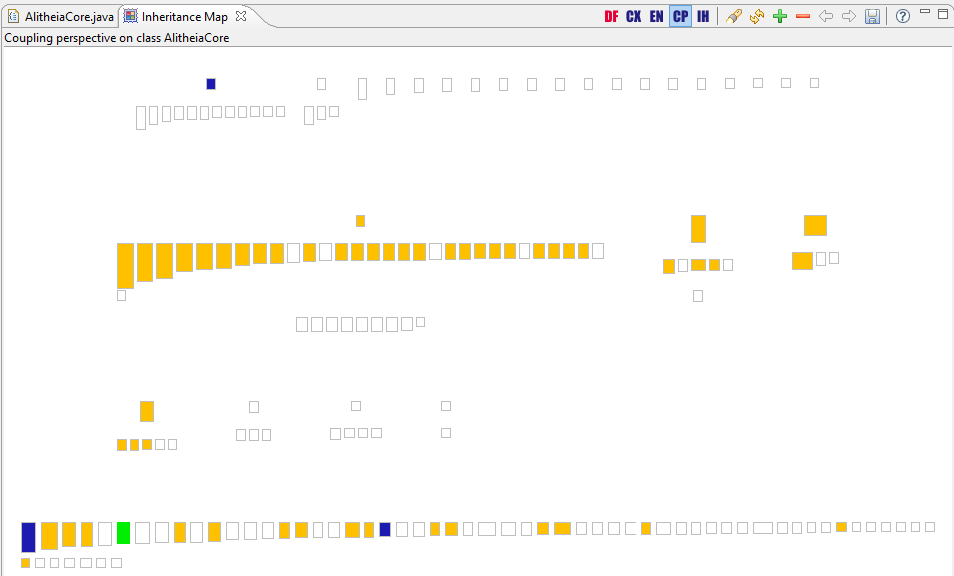
\includegraphics[width=0.8\textwidth]{alitheiacore-coupling}
    \caption{AlitheiaCore (green), its clients (yellow)}
    \label{fig:alitheiacore}
\end{figure}

From the inheritance map we observe that \verb|DAObject| (figure~\ref{fig:daobject}) and \verb|AlitheiaCoreService| (figure~\ref{fig:alitheiacoreservice}) have a lot of subclasses. The subclasses of \verb|AlitheiaCoreService| are interfaces for each service.

\begin{figure}[h]
\centering
\begin{minipage}{.45\textwidth}
  \centering
  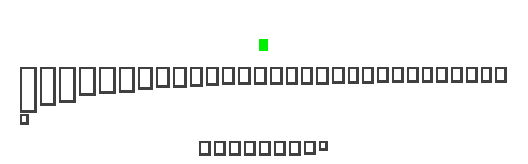
\includegraphics[width=0.9\linewidth]{daoobject-inheritance}
  \captionof{figure}{DAObject (green) and subclasses (bordered)}
  \label{fig:daobject}
\end{minipage}\hspace{5mm}%
\begin{minipage}{.45\textwidth}
  \centering
  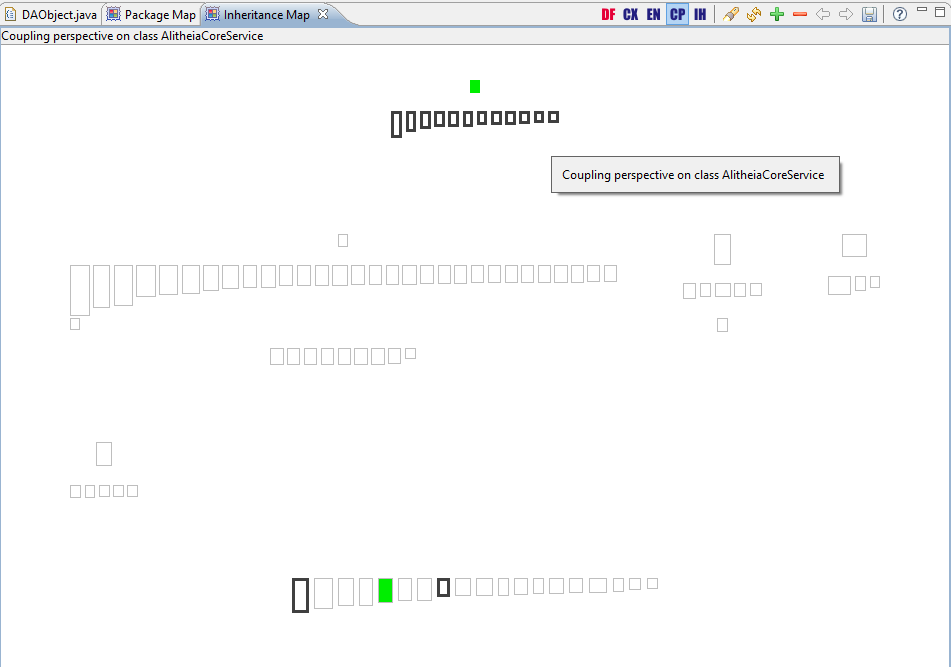
\includegraphics[width=0.9\linewidth]{alitheiacoreservice-inheritance}
  \captionof{figure}{AlitheiaCoreService (green) and subclasses (bordered)}
  \label{fig:alitheiacoreservice}
\end{minipage}
\end{figure}

A lot can be learned from the inheritance tree. We used IntelliJ IDEA 14~\footnote{https://www.jetbrains.com/idea/} to generate an inheritance diagram. Appendix~\ref{app:inheritance} contains the most important parts of the inheritance tree. From this tree, it is even more obvious that every service has an interface that extends \verb|AlitheiaCoreService|. For each of these interface an implementation exists in the package \verb|eu.sqooss.impl.service|. % zeg iets over DAObject

\section{Problem Detection}

\subsection{SRP violation}
\label{sec:srp}
\begin{enumerate}
\item The abstract class \verb|Job| contains a lot of methods. Its main responsibility is to represent the concept of a `job'. To accomplish this it contains properties (e.g. state, dependencies, dependees) and methods (addDependency, removeDependency, dependsOn) to alter its state. However, the class also exposes a method called verb|execute()|. This indicates that the \verb|Job| class is also responsible for executing a job. We argue that this is a violation of the SRP, because there is more than one motive for chaning the \verb|Job| class: either if the way we represent a job changes, or if the way we execute a job changes. A better architecture would be to move the job execution out of the \verb|Job| class and into a service layer (for example, \verb|JobExecuter|).

% Refs: www.objectmentor.com/resources/articles/srp.pdf, https://twitter.com/jeffrey_way/status/527857091470700544, http://verraes.net/2014/09/objects-as-contracts-for-behaviour/, http://msdn.microsoft.com/en-gb/magazine/dn385704.aspx, https://blog.inf.ed.ac.uk/sapm/2014/02/04/the-anaemic-domain-model-is-no-anti-pattern-its-a-solid-design/

\item The class \verb|ProjectsView.java|: its name suggests that it renders HTML output, but it also takes care of parsing the servlet's request object, adding projects, removing projects, and triggering updates.

\item Model classes should represent the corresponding domain entity, the whole domain entity and nothing but the domain entity. The class \verb|Bug| should represent a bug. It should not be aware of the way in which it is persisted (it should not be awere whether it is persisted at all). The current implementation of \verb|Bug.java| contains SQL queries for retrieving the information from the database and constructing the object, which is a major violation of the SRP principle.

% \item The ProjectEvent interface delcares a getEventPriority method and RepositoryEvent, MailingListEvent, and BugDBEvent implement this method. However, each class returns a constant. This indicates that event priority is actually not a property of these events. Diving a bit deeper we see that this method is used to compare ProjectEvent's. A correct way to implement this would be to create a custom comparator, which inspects the runtime type to compare two ProjectEvents. This is more extensible then returning integers (imaging creating an event that has property between two existing properties) and more maintainable.
\end{enumerate}

\subsection{OCP violation}
The \verb|Metric| class contains a property \verb|metricType: MetricType|. The \verb|MetricType| contains a \verb|Type| enumeration of types and a property \verb|type: String|. This indicates an overcomplicated design, because the \verb|MetricType| class does not add anything to the \verb|Type| enumeration (except the data access method \verb|getMetricType| that should not be there in the first place, see section~\ref{sec:srp}).

The \verb|Metric.java| class contains a method \verb|isEvaluated(StoredProject)|. This method contains a switch statements on a metric's type's enum type. Depending on the metric type's enum type, a different query is constructed. This is not open for modification, because we need to change the \verb|Metric| class if a new type is added in the future. To solve this issue, we suggest adding a \verb|isEvaluated(): String| method to a \verb|MetricType| interface from which all \verb|MetricType|'s must inherit. The \verb|isEvaluated(StoredProject)| method can then rely on the \verb|MetricType| interface.

We found this issue by searching for usages of `switch' in IntelliJ.

\subsection{LSP violation}
The class \verb|ProjectDirectory| inherits from \verb|ProjectFile|. However, not all properties that hold for \verb|ProjectFile| also hold for \verb|ProjectDirectory|. For example, whereas \verb|getFileName| would make sense for a \verb|ProjectFile|, it does not for a \verb|ProjectDirectory|.

We found this issue by inspecting the inheritance tree (see Appenidix~\ref{app:inheritance}). The fact that the subtyping does not establish an ``is-a'' relationship (i.e. a semantic relationship) indicates a possible violation of the LSP.

\subsection{DIP violation}
The class \verb|CacheServiceImpl| instantiates a subclass of itself. Being aware of your subclasses violates the DIP. The class should depend on abstractions instead of implementations.

The interface \verb|InMemoryCheckout| depends on the low level \verb|InMemoryDirectory| which is a violation of the Dependency Inversion Principle. % TODO: Uitbereiden, dit komt "overal" voor

\subsection{ADP violation}
% TODO: Define ADP in terms of packages?

We have searched for cyclic dependencies between packages using the `Analyze Cyclic Dependencies' feature in IntelliJ IDEA 14. A lot of interfaces in the package \verb|eu.sqooss.service| extend \verb|AlitheiaCoreService| in the package \verb|eu.sqooss.core|. These interfaces are also referenced in the \verb|AlitheiaCore| class. This means that the package \verb|eu.sqooss.service| depends on the package \verb|eu.sqooss.core| (via the \verb|AlitheiaCoreService| interface), but the \verb|eu.sqooss.core| package also depends on the \verb|eu.sqooss.service| package (via the \verb|AlitheiaCore| class), so this is an ADP violation.

% TODO: Insert graphic?

Besides that, a lot of classes in the package \verb|eu.squooss.impl.service| implement interfaces from the \verb|eu.sqooss.service| package. These are then bounded to these interfaces in the \verb|AlitheiaCore| class, so this is also an ADP violation.

\subsection{DRY violation}
In the class eu.sqooss.service.db.ProjectVersion a lot of duplicate is shared between the getLiveFilesCount and getVersionFiles methods. 

Furthermore, in the same class the methods getVersionByRevision and getVersionByTimestamp are exactly the same aside from one parameter.

% per principle:
% - wat het inhoud
% - hoe we gezocht hebben
% - wat we gevonden hebben

\subsection{Further examples}
We identified several code smells. We consider these smells less important than the SOLID violations discussed above. However, in order to maintain a high quality code base, we advice to address these smells and take appropriate measures.

\begin{enumerate}
\item The system uses \verb|AlitheiaCore| for providing implementations for certain interfaces, which is better than relying on implementations. However, this can be taken one step further by applying Inversion of Control (IoC)~\cite{ioc}. Instead creating your dependencies, you declare your dependencies and let someone higher up take care of creating them. This increases decoupling and makes maintaining code easier.

\item The code base contains commented code. See for example the \verb|createTestFiles| method in \verb|DiskUtil.java|, the \verb|static final int|'s you find above and below in that file. Also, \verb|Parser.java| is not used. We advice using a proper Version Control System (VCS) and only integrate production-code in the main branch.

\item Comments containing `TODO' or `FIXME'. Though this is not necessarily harmful, it is considered a better practice to store these in an issue tracker. An issue tracker provides others with an easy to grasp overview of existing issues. Furthermore, an issue tracker allows for more meaningful description's than ``this can break''.
\end{enumerate}

\bibliographystyle{plain}
\bibliography{report}

\newpage
\appendix
\section{Inheritance tree} \label{app:inheritance}

\begin{sideways}
	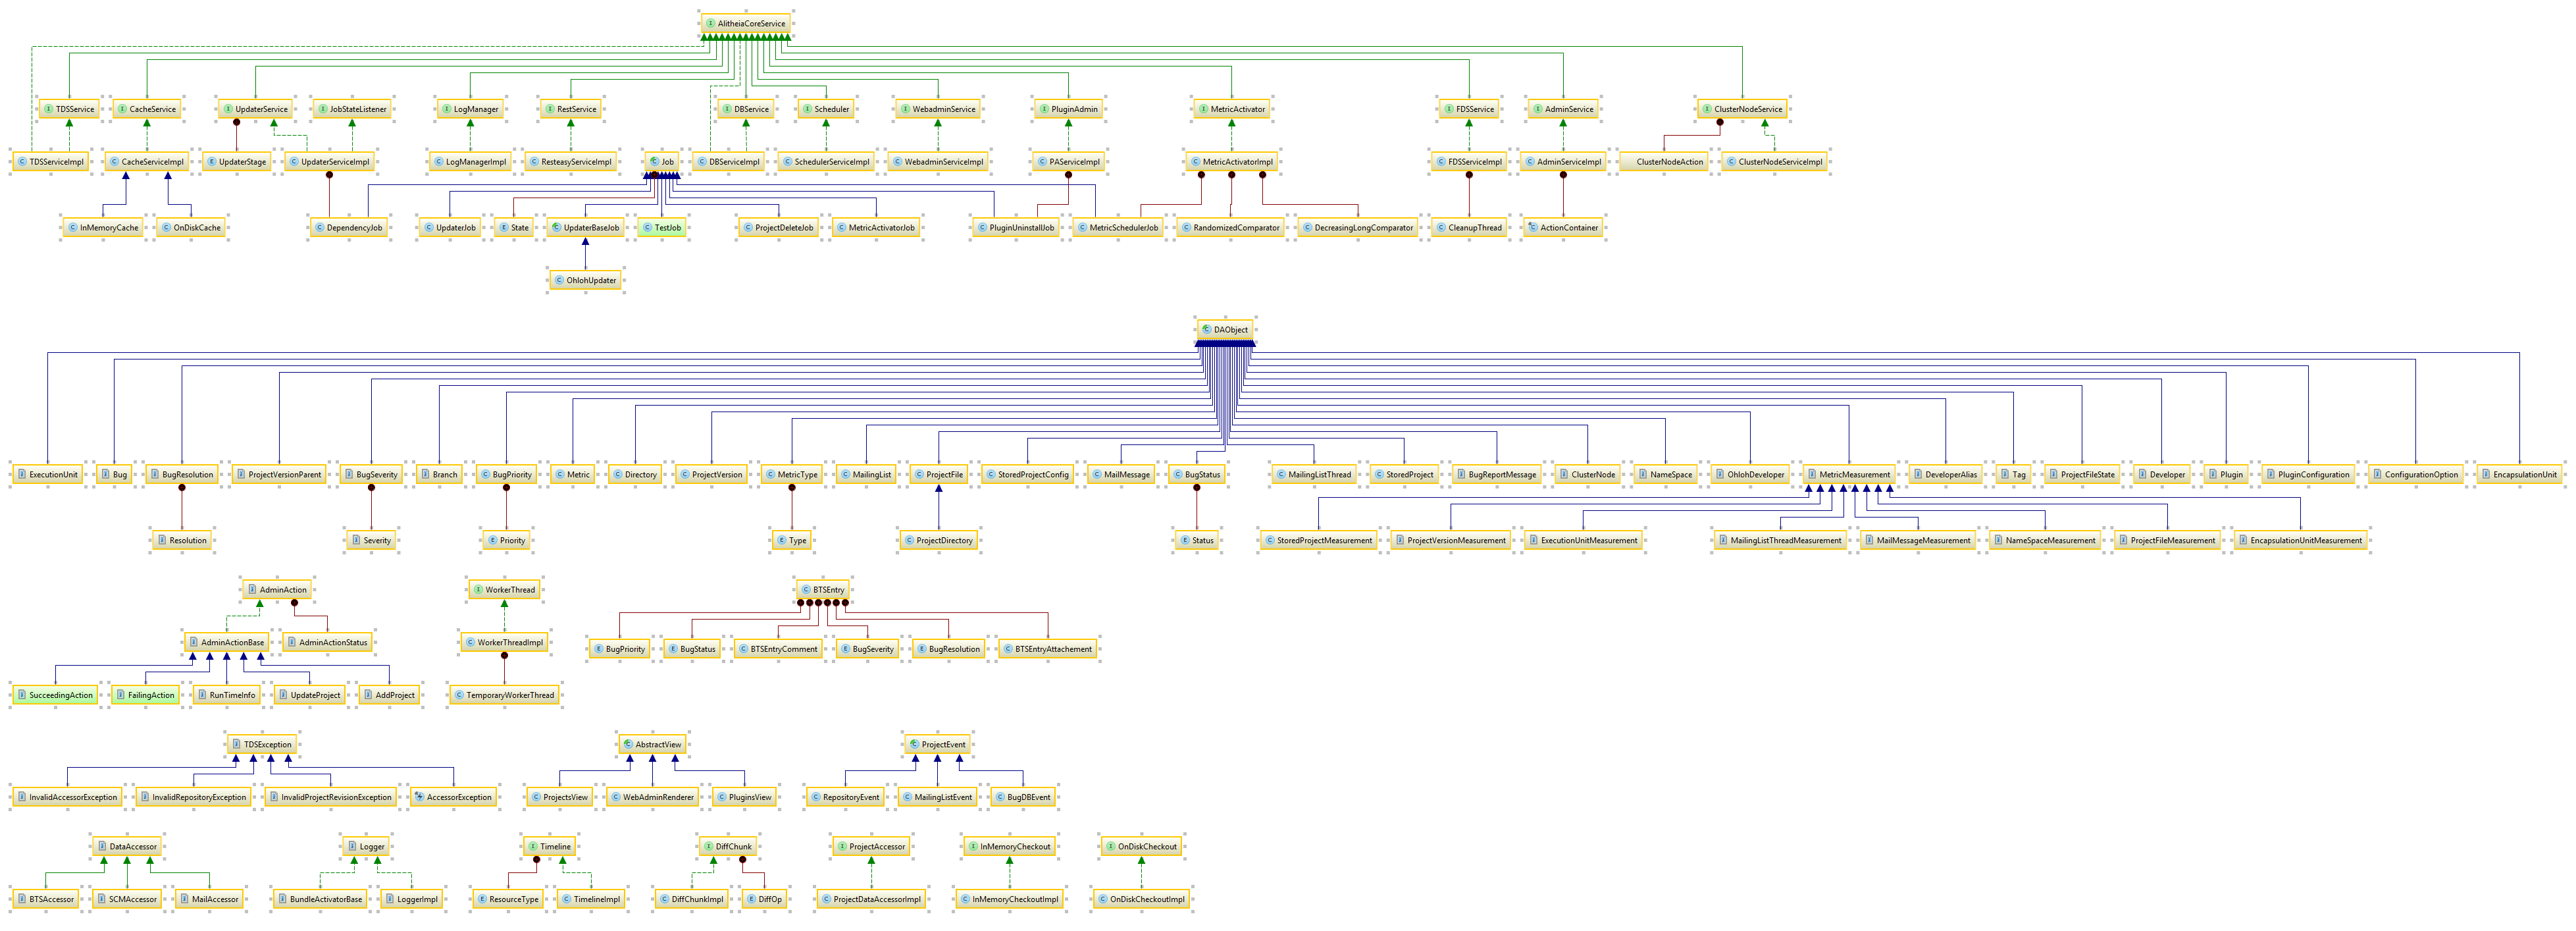
\includegraphics[width=1.3\textwidth]{inheritance-diagram}
	\label{fig:inheritance}
\end{sideways}

\end{document}